\chapter{Investigations}
We perform preliminary investigations into assessing the datasets for later formulating the appropriate methodology that would best suit their innate properties.

\section{Attribution of Comments}
 We seek an understanding of the strength of the association between comments and their authors, which is the first step towards our ultimate goal of comment-based models of author similarities.

Authorship attribution aims at predicting the writer of a given a piece of text. In general a variety of stylometric and lexical features are used. Authorship attribution problems generally arise in forensic settings, and involve relatively long documents, and lists of possible authors limited to a few hundred candidate authors. Often, a sizable amount of example text is available for each candidate.

In contrast, in our use case, the documents are short, the list of candidate authors is very large, and most are associated with little example text. The contribution of this paper is a first insight into how well commonly adopted authorship attribution techniques play out in a large candidate author set with short and informal text.

We aim to answer the following research questions:  
\begin{enumerate}
\item Can we predict an author of a comment from among a large number of candidates?
\item Which features aid in large-scale authorship attribution?
\item Are there differences between different communities of commenters (i.e., domains)?
\end{enumerate}

\subsection{Related Work}
%Most authorship attribution related research investigate either large documents or a smaller candidate author set or both.

Stamatatos provides an excellent summary of existing authorship attribution techniques \cite{stamatatos_survey_2009}. Most of the work discussed make use of both large documents and a smaller candidate author set. Stamatatos also points out that Support Vector Machines (SVM) perform extremely well as a distinguishing methodology in this particular scenario.

More recent work that looks into a smaller documents was done by Layton et al. \cite{layton_authorship_2010}, who look into authorship attribution for Twitter, where a micro-post (i.e., tweet) is restricted to 140 characters. Layton et al. opt for profile based feature representation of documents wherein all documents of a particular user are concatenated to form a super-document. They experiment with character $n$-grams with varying $n$ values and find that $4$-grams provide overall a good mean accuracy.

Work on large-scale attribution was carried out by Narayanan et al. \cite{narayanan_feasibility_2012}, who predict authors from a list of 100,000 candidate authors using a range of classifiers. Their dataset was comprised of blog posts, which are relatively longer than tweets or comments. They employed parts-of-speech tagging and a variety of lexical/character features for their purposes. A very interesting find in their work was that simple classifiers such as Naive Bayes and k-Nearest Neighbour performed better than SVM at the top ranks. 
%I took out this sentence because it breaks the flow.
%In addition, they make use of confidence estimation for the ranked list of classified authors rather than directly use the output of the classifier.

Our use case deals with shorter documents, namely comments, and a large candidate author set. We experiment with parts of methodologies adopted by Layton et al. \cite{layton_authorship_2010} and Narayanan et al. \cite{narayanan_feasibility_2012} as our problem is a combination of both. The upcoming sections discuss our methodology and the results of our experiments.

\subsection{Method}
In our scenario, the training set is highly imbalanced, with a vast majority of authors having made very few comments and a handful of authors who made thousands of comments. For this reason, we adopt instance-based classification, wherein each document contributes on its own to the attribution and choose a simple k-NN classifier.

The features we make use of are the frequency counts of character $n$-grams similar to that of Layton et al., since our use case also deals with similar informal text and shorter documents. We experiment with different values of $n$. We expect the value of $n$ to be important, since our data sets are not homogeneously mono-lingual. We perform a basic thresholding by selecting only those $n$-grams that occur more than three times in the entire dataset.

%so as to eliminate any artifacts that would potentially bring down the performance of the classifier.
%The problem is that infrequently occurring words do not allow generalization.

The character $n$-gram frequency is converted into a feature vector and fed into the k-NN classifier. For a given unknown comment, the classifier outputs nearest neighbour comments, which are labeled with authors. In essence, our method makes a prediction based on documents using similar vocabulary as our target document.

\subsection{Experiments}
SC comments are very short whereas NU comments are relatively longer. It also goes without saying both are different domains and cater to different audiences. We performed basic spam filtering for SC by removing all comments that contained the literal `$http$' (naive url filtering) as these would produce $n$-gram artifacts and were possibly created by bots. NU is strictly moderated and the possibility of occurrence of spam is low.

We partition the data temporally: the first 11 months of comments are taken as the training set and the last month as the test set. This partitioning was chosen since we are interested in predicting authorship based on historical data, and in any real world scenario, one can only predict future behaviour based on past instances and not the other way around. We also take into consideration only the candidate authors who had made at-least six comments, since we assume that it is not possible to make predictions with less data. Table~\ref{tab:split} shows the underlying split of data.

\begin{table}[]
\centering
\begin{tabular}{|l|c|c|c|c|}
\hline
 \textbf{Dataset} & \textbf{Train/Test} & \textbf{No. of Users} & \textbf{No. of Comments} & \textbf{Avg. Comment Length} \\ \hline
 \multirow{2}{*} {SC} &  Train & 15,665 & 558,909 & 47.35 chars\\ \cline{2-5}
 & Test & 15,665 & 152,335 & 44.61 chars\\ \hline
 \multirow{2}{*}{NU} & Train & 11,958 & 1,067,451 & 245.11 chars\\ \cline{2-5}
 & Test & 11,958 & 175,433 & 233.48 chars\\ \hline
\end{tabular}
\caption{Data Split}
\label{tab:split}
\end{table}

The metric we use for evaluation is Mean Reciprocal Rank (MRR) which is %essentially 
the average of the reciprocal rank of the first hit in the list of candidates. We compute RR for those instances in which the author is found in the top 100 ranked results. For the rest of the cases, we assume that the author was ranked at infinity, and these cases contribute a RR of zero to the MRR. We also make use of $A@N$ which represents the accuracy at or less than rank N, i.e., percent of comments in the entire set that were correctly classified at or less than rank N.

As a sanity check, we calculated a trivial baseline that drew a comment from the training set at random. In essence, the baseline prioritizes users who have made more comments. The baseline had an $MRR < 0.001$ in both cases of NU and SC.

Table~\ref{tab:com_results} shows the results of classification averaged over all comments. 
Overall NU is a more challenge use scenario than SC. 
For the case of SC, $2$-grams perform best and $3$-grams slightly better than $2$-grams for the case of NU with $4$-grams performing the worst for both cases.

\begin{table}[!h]
\centering
\begin{tabular}{|l|c|c|c|c|c|}
\hline
 \textbf{Dataset} & \textbf{n-gram} & \textbf{MRR} & \textbf{A@1} & \textbf{A@5} & \textbf{A@10}\\ \hline
 \multirow{3}{*}{SC} & \textbf{2} & \textbf{0.1176} & \textbf{8.94} & \textbf{14.43} & \textbf{17.18}\\ \cline{2-6}
 & 3 & 0.1090 & 8.51 & 13.25 & 15.53\\ \cline{2-6}
 & 4 & 0.1000 & 7.79 & 12.22 & 14.35\\ \hline
 \multirow{3}{*}{NU} & 2 & 0.0321 & 1.96 & 4.05 & 5.48\\ \cline{2-6}
 & \textbf{3} & \textbf{0.0341} & \textbf{2.23} & \textbf{4.32} & \textbf{5.59}\\ \cline{2-6}
 & 4 & 0.0254 & 1.71 & 3.16 & 4.12\\ \hline
\end{tabular}
\caption{Per-Comment Results}
\label{tab:com_results}
\end{table}

We attribute the difference of performance between SC and NU to the temporal evolution of the vocabulary of NU. SC users consistently utilize more or less the same vocabulary over time whereas those of NU necessarily do not. NU comments could be expected to change vocabulary since NU is a news dataset, and news topics change over time. For instance, during the month of December, Christmas and New Year were popular topics and there were numerous usages of keywords related to these topics.
%whereas during other months there were varying topics depending on what was trending. 
SC on the other hand does not have these drastic changes, since people are commenting on music, for which, unlike news, the topics do not rapidly change or evolve over time.

As for the particular performance of $n$-grams, we assume that $4$-grams performed worst because they were too specific. In the case of NU, there is only a marginal difference between $2$-grams and $3$-grams. For SC, $2$-grams performed best, explainable by the short length of SC comments, but also by the fact that they are
%which may be attributed to the fact that the average SC comment has a very short length. 
 often filled with emoticons and punctuation, which are at most times shorter than lexical words.

Figure~\ref{fig:sc_feat_mrr} and Figure~\ref{fig:nu_feat_mrr} further explore whether the number of $n$-grams in each comment affected the final MRR score. Specifically, we investigate whether the length of the comment affects the MRR. For the sake of observation, we divide the dataset into equally distributed 5\% quantiles based on the $n$-gram count and find the mean of all MRR scores within the bounds of these quantiles. A fit over the distribution is then made, and is referred to as the Quantile Bounded Mean ($QBM$).

We only look into the $n$-grams that performed best for SC and NU ($n$=2,3). We limited the graphs up till the $99^{th}$ quantile, since we assumed that going beyond that would take into consideration outliers that would not be very informative for our purposes. 
%This next sentence, it is very nice that you say this, but conventionally people don't explicitly point it out. It confused me when I first read it, so I think it is better to leav it out.
%It is also to be noted that we have scaled down the MRR to 0.4 for both graphs for better clarity.

\begin{figure}[!h]
\centering
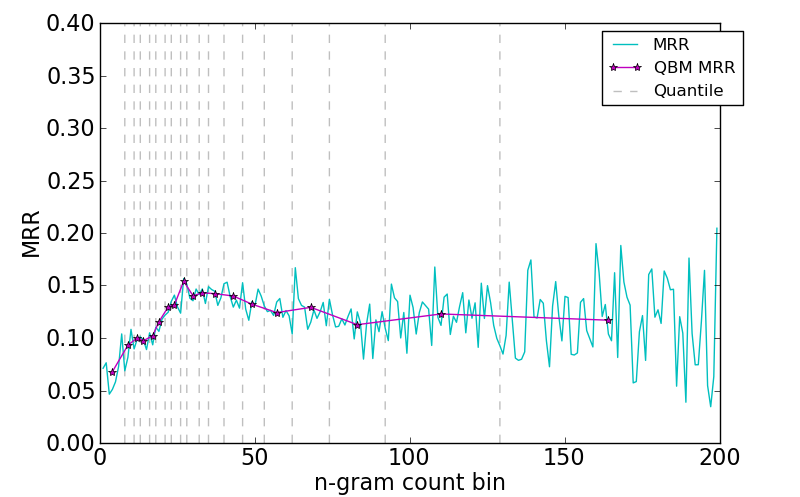
\includegraphics[width=0.6\textwidth]{c-3_images/sc_feat_mrr.png}
\caption{MRR vs $2$-gram counts for SC}
\label{fig:sc_feat_mrr}
\end{figure}

\begin{figure}[!h]
\centering
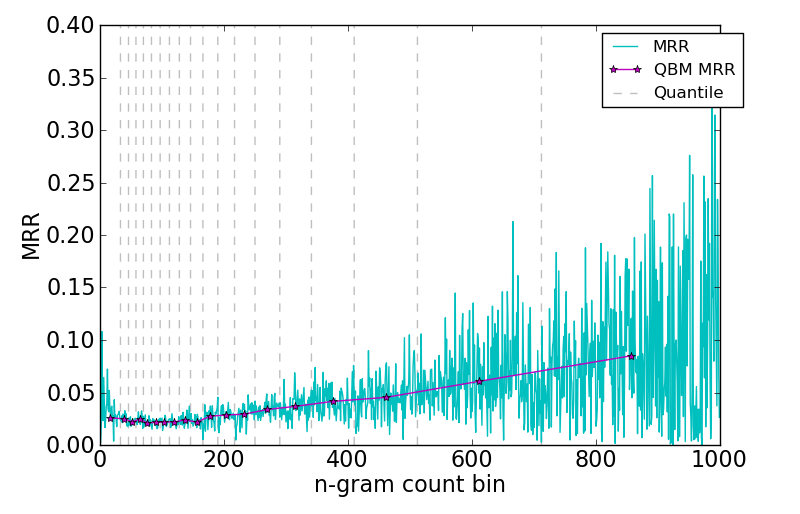
\includegraphics[width=0.6\textwidth]{c-3_images/nu_feat_mrr.png}
\caption{MRR vs $3$-gram counts for NU}
\label{fig:nu_feat_mrr}
\end{figure}

Interestingly, for the case of SC, the MRR peaks early on, and then slightly decreases before finally leveling off. A common behavior observed in SC was that different users often used the same vocabulary, for instance the exact same comment `nice' alone occurred 560 times in the dataset. This behavior explains the particularly low value in the case of shorter comments. 
% This sentence doesn't make sense. If long comments promote content, and use the same words to do so, then the performance should go up. I would just leave it out.
%The longer comments were often comprised of users promoting content or plain spam explaining the decrease and stagnation over time.

In the case of NU, the length of the comment is proportional to the MRR. Although there are wide variations towards longer comments overall the mean gradually increases.

\subsection{Conclusion and Outlook}
%I moved this to the beginning, because usually the conclusion comes before the outlook to future work.
By use of a simple experimental setup, we were able to examine two similar, but at the heart very different, datasets. In spite of a large candidate author set and smaller document size, we were able to make correct predictions in about 15\% of the cases for SC. Our conclusion is that large scale attribution is to an extent domain dependent, and that it is possible with the right features.

%Not spam filtering! You would have to show that spammer's behavior is not actually helping you in order to say that. It's feature selection, thaty ou mean. I changed it.
We believe that if more sophisticated feature selection techniques were adopted, there would be additional improvement in performance. 
Our experiments raise the question of how redundant comments such as `nice' can be characterized. 
In our future work, we will address this question by investigating the introduction of the context of the item into the picture. 
% I am suggesting to leave out the remarks about the co-commenters. Ultimately you are actually trying to predict commenter similarities (the intro now states this), so you don't want to put too much emphasis on this point here.
%We hypothesize that comments aid in characterizing the item, therefore co-occurring comments could potentially act as a medium for attributing the target author's own comment. 
Meta features such as the time of the day the target user frequently comments, or geo-graphic location of the commenter could also be helpful.
%or the co-commenters the target user consistently comments beside with similar to that of a collaborative filtering scenario might also prove helpful.

NU on the other hand is an entirely different situation altogether: there are not as many repeated $n$-grams. In addition, users are reacting to ever-changing topics, and it could be helpful to supplement $n$-grams with other features. If one were to make use of conventional authorship features such as text compression, parts-of-speech, lexical features (frequency of punctuation, word length, sentence length), which capture subtle stylometric features rather than just the text, one might see an improvement over the base performance. It is open to question whether the context of the item would be helpful considering the rapid change in topic contrary to SC. Since NU largely caters to an audience of a single region, the time- and location-based meta features might not be as helpful.

In addition, we also evaluated the prediction by utilizing the id's of the co-commenters of the target user in the training set in contrast to utilizing only the target user's id as previously adopted. The results are presented in Table~\ref{tab:co_results}

\begin{table}[!h]
\centering
\begin{tabular}{|l|c|c|}
\hline
 \textbf{Dataset} & \textbf{Classifier} & \textbf{MRR} \\ \hline
 \multirow{8}{*}{SC} 
 & Baseline & 0.0806 \\ \cline{2-3}
 & 2-gram kNN & 0.3259 \\ \cline{2-3}
 & 3-gram kNN & 0.3143 \\ \cline{2-3}
 & 4-gram kNN & 0.3046 \\ \cline{2-3}
 & 99\% Baseline & 0.0770 \\ \cline{2-3}
 & 99\% 2-gram kNN & 0.2741 \\ \cline{2-3}
 & 99\% 3-gram kNN & 0.2656 \\ \cline{2-3}
 & 99\% 4-gram kNN & 0.2551 \\ \hline
 \multirow{8}{*}{NU} 
 & Baseline & 0.5636 \\ \cline{2-3}
 & 2-gram kNN & 0.7953 \\ \cline{2-3}
 & 3-gram kNN & 0.7908 \\ \cline{2-3}
 & 4-gram kNN & 0.7783 \\ \cline{2-3}
 & 99\% Baseline & 0.5550 \\ \cline{2-3}
 & 99\% 2-gram kNN & 0.7048 \\ \cline{2-3}
 & 99\% 3-gram kNN & 0.7056 \\ \cline{2-3}
 & 99\% 4-gram kNN & 0.7017 \\ \hline
\end{tabular}
\caption{Results Evaluated with Co-Commenter Labels as Ground Truth}
\label{tab:co_results}
\end{table}

In both datasets, there were outlier co-commenters who made a very large number of comments  around 9k in the case of NU and  around 4k in the case of SC. This would lead to a free lunch scenario where every target user has this outlier user as a co-commenter. Therefore, we limit our co-commenter evaluation up till the $99^{th}$ percentile of number of comments in the dataset. Explicitly setting a threshold of <357 for SC and <944 for NU, these results are shown prepended with 99\%.

In addition, we also employ the previous baseline which made random predictions while prioritizing users who made higher number of comments. As can be seen, users of NU consistently co-comment with each other inferring from the random baseline. There is very slight difference between 2-gram and 3-gram features but overall this also gives insight that users who consistently co-comment make use of the same words. Our earlier observation was that a single user does not use of the same words over time but this leads us to believe that there is a predominant pattern among different users that leads them to co-comment and also make use of relatively the same words.

SC on the otherhand does not have the same behaviour as NU, this indicates that the community of SC is more fragmented than that of NU as the baseline is inferior compared to that of NU. But, relativistic to the baseline 2-gram features perform better. But in comparison to the earlier single user results, there is no drastic change as observed in NU. One of the reasons might be that there is too much redundancy in the words used by the user that it makes very slight difference to evaluate with respect to the co-commenters.